\documentclass[11pt,a4paper]{report}

\usepackage[margin={1cm,2cm,1cm,2cm}]{geometry}
\usepackage[T2A]{fontenc}
\usepackage[utf8]{inputenc}
\usepackage[russian]{babel}
\usepackage{cmap}
\usepackage{amsmath,amsfonts}
\usepackage{graphicx,color}
\usepackage[makeroom]{cancel}
\usepackage{rotating}
\usepackage{feynmp-auto,tikz}
\usepackage{subfigure,float}
\usepackage{hyperref}
\hypersetup{colorlinks=false}

\input{diagrams}

\begin{document}

%%% Maketitle metadata
\newcommand{\horrule}[1]{\rule{\linewidth}{#1}}   % Horizontal rule

\title{
  \vspace{-1in}
  \normalfont \normalsize \textsc{Московский Государственный Университет} \\ [25pt]
  \horrule{0.5pt} \\[0.4cm]
  \huge Диаграммные методы в сильно коррелированных электронных системах \\
  \horrule{2pt} \\[0.5cm]
}
\author{
  \normalfont
  \normalsize
  {Николай А. Мурзин}\\[-3pt]
  \normalsize
  {\it{науч. рук.:} \normalfont{Алексей Н. Рубцов}}\\[-3pt]
  \normalsize
}
\date{\today}
\maketitle
\tableofcontents

\chapter{Обзор}

\section{Введение}

Сильно коррелированные электронные системы содержат в себе наиболее интригующие эффекты физики конденсированного состояния, такие как высоко температурную сверхпроводимость, 
поведение тяжелых фермионов, аномальный Кондо эффект, различные виды электронных фазовых переходов и многое многое другое\cite{anderson1984basic}\cite{anderson1997theory}\cite{scalapino1995case}\cite{hewson1997kondo}.
Существенно описание большого числа частиц с очень сильными для обычной теории возмущений корреляциями. В связи со сложностью задачи, физика сильно коррелированных систем представляет из себя теоретически очень привлекательную область.
Одним из удачных путей описания является Теория Динамического Среднего Поля (DMFT)\cite{georges1996dynamical}\cite{kotliar2004strongly}. Обще принято что этому подходу удается уловить большинство существенных корреляционных эффектов, например поведение
переходов металл-изолятор Мотт-Хаббарда\cite{mott1974metal}. Метод был успешно внедрен в вычисления реальных электронных структур\cite{anisimov1997first}\cite{lichtenstein1998ab}, которые уже являются стандартным средством в микроскопической теории сильно коррелированных систем.
Тем не менее существует множество эффектов, для которых не локальные корреляции выходят на первый план и часто наиболее важными являются корреляции именно дальнего порядка. 
Например образование жидкости Люттингера в мало размерных системах\cite{anderson1997theory}\cite{mahan2000many}, поведение нефермиевской жидкости с сингулярностями Ван-Хова на плоскости\cite{irkhin2001effects}\cite{irkhin2002robustness},
физика около критических точек или d-волны ВТСП\cite{scalapino1995case}.

DMFT берет в рассмотрение локальные динамические корреляции, но пренебрегает внутри-узловыми корреляциями, что отражено в независимости собственной энергии от $\mathbf{k}$: $\Sigma_\mathbf{k}\equiv \Sigma_{\text{loc},\omega}$. 
Теории возмущений, такие как теория T-матриц, обмен флуктуациями (fluctuation exchange, FLEX) и паркетные приближения\cite{bickers} могут привести к $\mathbf{k}$-зависимой $\Sigma$,
но наиболее важные локальные корреляции не воспроизводятся в режиме слабой связи, когда параметр $U$ кулоновского взаимодействия сравним или больше ширины зоны.
Для учета флуктуационных локальных корреляций необходима диаграммная техника, строящаяся поверх DMFT.

Одним из методов включения пространственных корреляций служит диаграммный Метод Дуальных Фермионов (DF)\cite{PhysRevB.77.033101}. Он основан на введении новых переменных в представлении интеграла по траекториям.
Этот подход приводит к удовлетворительным результатам уже в низших порядках возмущений по сравнению с DMFT, например уменьшению критической температуры антиферромагнитной нестабильности в модели Хаббарда 
при полузаполнении\cite{PhysRevB.77.195105}. Введение новых дуальных переменных позволяет включить локальный вклад к собственной энергии в дуальную функцию Грина и достичь быстрой сходимости в ряде возмущений.

Существуют и другие диаграммные техники, метод $D\Gamma A$\cite{toschi2007dynamical}\cite{katanin2009comparing} и относительно новый метод 1PI\cite{katanin}. 
В этой работе делается сравнение DF и 1PI методов на примере двух диаграмм третьего порядка, приводятся численные результаты для двухмерной модели Хаббарда в режиме с полузаполнением.

\section{Формализм дуальных фермионов}
Задача состоит в поиске приближенного решения для обобщенной задачи с действием

\begin{equation}
\label{action}
 S\left[c^*,c\right] = - \sum_{\omega\mathbf{k}\sigma m m'} c^*_{\omega\mathbf{k}\sigma m} ((i\omega+\mu)\mathbf{1}-h_{\mathbf{k}\sigma})_{m m'}c_{\omega\mathbf{k}\sigma m'} + \sum_i H_{int}[c_i^*,c_i]
\end{equation}

Здесь $h_{\mathbf{k}\sigma}$ - одноэлектронная часть Гамильтониана, $\omega_n=(2n+1)\pi/\beta,n = 0,\pm 1,\dots$ - фермионные Мацубаровские частоты, 
$\beta$ и $\mu$ - обратная температура и химический потенциал соответственно, $\sigma=\uparrow,\downarrow$ - спиновые индексы,
$m,m'$ - орбитальные индексы, $i$ - индексирует узлы решетки, $\mathbf{k}$ - вектор квазимомента, а $c^*$,$c$ - Грасмановы переменные. 
$H_{int}$ может быть любым типом взаимодействия. Единственное ограничение, что оно локально в пределах атома или кластера. Кулоновское взаимодействие например

\begin{equation}
 H_{\text{int}}[c^*_i,mc_i] = \frac{1}{4} \int_0^\beta \mathrm{d}\tau U_{1234} c_{i1}^* c_{i2}^* c_{i3} c_{i4}
\end{equation}

Где $U$ - сила кулоновского взаимодействия, а индексы (\textit{напр.} $1\equiv{\omega_1 m_1\sigma_1}$) вмещают частотные, орбитальные и спиновые состояния, по которым производится суммирование.

Идея техники дуальных фермионов заключается в переформулировке решеточной задачи в терминах невзаимодействующих примесей, а взаимодействие перенесено на второстепенные частицы.
Как и в теории динамического среднего поля (DMFT), вводится действие для локальной примеси в виде

\begin{equation}
 S_{\text{imp}}[c^*,c] = - \sum_{\omega\sigma m m'}c^*_{\omega\sigma m}((i\omega+\mu)\mathbf{1}-\Delta_{\omega\sigma})_{mm'}c_{\omega\sigma m'} + H_{int}[c^*,c]
\end{equation}

Где $\Delta$ - пока неизвестная матрица гибридизации, описывающая взаимодействие между примесью и термостатом.

Из-за локальности $\Delta$ возможно расцепление взаимодействующих узлов и действие \ref{action} можно переписать как

\begin{equation}
 S[c^*,c] = \sum_i S_{\text{imp}}[c^*_{\omega i \sigma m'},c_{\omega i\sigma m}] - \sum_{\omega\mathbf{k}\sigma mm'}c^*_{\omega\mathbf{k}\sigma m}(\Delta_{\omega\sigma}-h_{\mathbf{k}\sigma})_{mm'}c_{\omega\mathbf{k}\sigma m'}
\end{equation}

Дуальные фермионы вводятся при помощи преобразования Хаббарда-Стратоновича, выполняющееся для произвольных комплексных матриц $\hat(A)$ и $\hat{B}$

\begin{equation}
 \int \exp{(-\mathbf{f}^*\hat{A}\mathbf{f}-\mathbf{f}^*\hat{B}\mathbf{c}-\mathbf{c}^*\hat{B}\mathbf{f})}\mathcal{D}[\mathbf{f}^*,\mathbf{f}] = \det{(\hat{A})}\exp{(\mathbf{c}^*\hat{B}\hat{A}^{-1}\hat{B}\mathbf{c})}
\end{equation}

Выбирая 
\begin{equation}
\begin{split}
 A &= g_{\omega\sigma}^{-1}(\Delta_{\omega\sigma}-h_{\mathbf{k}\sigma})^{-1} g_{\omega\sigma}^{-1} \\
 B &= g_{\omega\sigma}^{-1}
\end{split}
\end{equation}

Где $g_{\omega\sigma}$ - локальная функция Грина примеси. В итоге получаем

\begin{equation}
 S[\mathbf{c}^*,\mathbf{c},\mathbf{f}^*,\mathbf{f}] = \sum_i S_{\text{site},i} + \sum_{\omega\mathbf{k}\sigma}
 \left[\mathbf{f}^*_{\omega\mathbf{k}\sigma} g_{\omega\sigma}^{-1}(\Delta_{\omega\sigma}-h_{\mathbf{k}\sigma})^{-1} g_{\omega\sigma}^{-1}\mathbf{f}_{\omega\mathbf{k}\sigma}\right]
\end{equation}

Таким образом взаимодействие между узлами заменилось на взаимодействие с дуальными фермионами

\begin{equation}
 S_{\text{site},i} = S_{\text{imp}}[\mathbf{c}^*,\mathbf{c}] + \mathbf{f}^*_{\omega i\sigma} g_{\omega\sigma}^{-1}\mathbf{c}_{\omega i\sigma} + \mathbf{c}^*_{\omega i\sigma} g_{\omega i\sigma}^{-1}\mathbf{f}_{\omega i\sigma}
\end{equation}

Где из-за локальности $g_{\omega\sigma}$, сумму по $\mathbf{k}$ можно заменить на сумму по узлам.

Теперь возможно проинтегрировать первоначальные фермионы для каждого узла в отдельности

\begin{equation}
 \int \exp{(-S_{\text{site}}[\mathbf{c}^*_i,\mathbf{c}_i,\mathbf{f}^*_i,\mathbf{f}_i])}\mathcal{D}[\mathbf{c}^*_i,\mathbf{c}_i] = Z_{\text{imp}} e^{(-\sum_{\omega\sigma}\mathbf{f}^*_{\omega i\sigma}g_{\omega\sigma}^{-1}\mathbf{f}_{\omega i\sigma}+V_i[\mathbf{f}^*_i,\mathbf{f}_i])}
\end{equation}

Раскладывая обе части этого уравнения и приравнивая соответствующие порядки малости, получаем

\begin{equation}
 V[\mathbf{f}^*,\mathbf{f}] = -\frac{1}{4} \gamma_{1234}^{(4)}\mathbf{f}^*_{1}\mathbf{f}_{2}\mathbf{f}^*_{3}\mathbf{f}_{4} + 
 \frac{1}{36} \gamma_{123456}^{(6)}\mathbf{f}^*_{1}\mathbf{f}_{2}\mathbf{f}^*_{3}\mathbf{f}_{4}\mathbf{f}^*_{5}\mathbf{f}_{6} + \dots
\end{equation}

Где $\gamma^{(4)}$ - неприводимая двух-частичная вершина решеточных фермионов

\begin{equation}
\begin{split}
 \gamma_{1234}^{(4)} &= g_{11'}^{-1}g_{22'}^{-1}\left[\chi_{1'2'3'4'}^{\text{imp}}-\chi_{1'2'3'4}^{\text{imp},0}\right]g_{33'}^{-1}g_{4'4}^{-1} \\
 \chi_{1234}^{\text{imp},0} &= g_{14}g_{23} - g_{13}g_{24}
\end{split}
\end{equation}

, $g$ - локальная функция Грина примесной задачи, $\chi$ - локальная двух-частичная функция Грина примесной задачи

\begin{equation}
 \chi_{1234}^{\text{imp}} = \frac{1}{Z_{\text{imp}}} \int \mathbf{c}_1 \mathbf{c}_2 \mathbf{c}^*_3 \mathbf{c}^*_4 \exp{(-S_{\text{imp}}[\mathbf{c}^*,\mathbf{c}])}\mathcal{D}[\mathbf{c}^*,\mathbf{c}]
\end{equation}

В результате дуальное действие после интегрирования по решеточным фермионами

\begin{equation}
 \label{dual_S}
 \tilde{S}[\mathbf{f}^*,\mathbf{f}] = -\sum_{\omega\mathbf{k}\alpha\beta}\mathbf{f}^*_{\omega\mathbf{k}\alpha}[\tilde{G}^{(0)}_{\omega\sigma}(\mathbf{k})]_{\alpha\beta}^{-1}\mathbf{f}_{\omega\mathbf{k}\beta}+\sum_i V_i[\mathbf{f}^*_i,\mathbf{f}_i]
\end{equation}

Где дуальная функция Грина

\begin{equation}
 \label{dual_G}
 \tilde{G}^{(0)}_\omega(\mathbf{k}) = -g_\omega\left[g_\omega+(\Delta_\omega-h_\mathbf{k})^{-1}\right]^{-1} g_\omega
\end{equation}

До этого момента уравнения (\ref{dual_S}) и (\ref{dual_G}) являются лишь переформулировкой первоначальной задачи. На практике же приближенные решения получаются из возмущения дуальной задачи.
Несколько диаграмм дающие вклад в собственную энергию показаны на рисунке \ref{diags}. Диаграммы сконструированы из примесных вершин и дуальных функция Грина в качестве линий.

После расчета приближенной собственной энергии, результат может быть переведен обратно в терминах решеточных фермионов используя точные соотношения. 
Абстрактная природа дуальных переменных может создать впечатление произвольности и неконтроллируемости приближений в разложении в ряд дуального потенциала, 
 но можно показать, что приближения могут быть сконструированы из физических соображений, как и в обычном случае.

\section{Дуальная теория возмущений}

Действие (\ref{dual_S}) ведет к созданию диаграммной техники по степеням дуального потенциала $V$. В конечном итоге можно прийти к правилам построения диаграмм для собственной энергии в импульсном пространстве
 
\begin{itemize}
 \label{rules}
 \item Рисуются все топологически различные, соединенные диаграммы, включающие в себя любые $n$-частичные взаимодействия $\gamma^{(2n)}$, изображаемые в виде правильных многоугольников с $2n$ концами, 
 $n$ исходящими с исходящей направленной линией и соответственно $n$ входящими
 \item все концы вершин соединяются направленными линиями, в соответствии с исходящим или входящим типом
 \item в соответствие каждой линии ставится дуальная функция Грина $\tilde{G}$
 \item Расставляются частоты, импульсы, орбитальные и спиновые индексы для каждого конца вершины, принимая в расчет законы сохранения энергии, импульса и спина
 \item Суммируются/интегрируются все внутренние переменные
 \item Для каждого набора $n$ эквивалентных линий (одинаково направленных и соединяющих одни и те-же концы) ставится фактор $1/n!$
 \item Результат умножается на фактор $(T/N)^m S^{-1}$, где $m$ - число независимых сумм по частотам/импульсам, а $S$ - фактор симметрии\cite{negele1998quantum}
 \item Для диаграмм, содержащих только двух-частичные взаимодействия, знак определяется заменой квадрата линией вертикального взаимодействия и считается число образовавшихся циклов $n_l$. Знак равен $(-1)^{n_l}$.
\end{itemize}
 
Закону сохранения энергии соответствуют $\delta$-функции $\delta(\omega_1+\omega_3+\dots+\omega_{2n-1}-\omega_2-\omega_4-\dots-\omega_{2n})$ в каждой вершине.
Число $m$ независимых суммирований остается после интегрирования всех этих $\delta$-функций. $T = \beta^{-1}$ - температура, $N$ - число $k$-точек в первой зоне Брюллиэна.
 
\begin{figure}[H]
\label{diags}
\centering
\subfigure[\label{fig:diag0}]{\diagzero}
\subfigure[]{\diagtwoG}
\subfigure[]{\diagthreeGempty}
\subfigure[]{\begin{tikzpicture}[baseline=-35pt]{\node{\diagsixempty};}\end{tikzpicture}}
\caption{Диаграммы}
\end{figure}

\section{Дуальная вершина}

\begin{figure}[H]
\centering
\diagvertex
\caption{Дуальная вершина}
\end{figure}

Дуальная вершина вычисляется из уравнения Бете-Солпитера
\begin{equation}
\Gamma_{\substack{\Omega K\\ \omega\omega'}}^\alpha = \gamma^\alpha_{\substack{\Omega\\ \omega\omega'}} 
  - \beta^{-1} \sum_{\omega''}\gamma_{\substack{\Omega\\ \omega\omega''}}^\alpha
    \overbrace{\left(\int_k \tilde{G}_{\substack{\Omega+\omega''\\K+k}}\tilde{G}_{\substack{\omega''\\k}}\right)}^{-\tilde{\chi}^{(0)}_{\substack{\Omega K\\\omega''}}}
    \Gamma_{\substack{\Omega K\\\omega''\omega'}}^\alpha
\end{equation}
Здесь $\alpha=d,m$ -  электрон-дырочный канал плотности и магнитный канал

\begin{equation}
\begin{split}
  \Gamma_{\substack{\Omega\\ \omega\omega''}}^d =  \Gamma_{\substack{\Omega\\ \omega\omega''}}^{\uparrow\uparrow\uparrow\uparrow} + \Gamma_{\substack{\Omega\\ \omega\omega''}}^{\uparrow\uparrow\downarrow\downarrow} \\
  \Gamma_{\substack{\Omega\\ \omega\omega''}}^m =  \Gamma_{\substack{\Omega\\ \omega\omega''}}^{\uparrow\uparrow\uparrow\uparrow} - \Gamma_{\substack{\Omega\\ \omega\omega''}}^{\uparrow\uparrow\downarrow\downarrow}
\end{split}
\end{equation}

Физическое содержание уравнения БС состоит в повторении рассеяния пар частица-дырка. В этих двух каналах пара частица-дырка имеет определенный полный спин $S$ и проекцию спина $S_z$.
Канал плотности соответствует $S=0$, $S_z=0$ синглетному каналу, а вершина $\Gamma^m$ соответствует $S=1$, $S_z=0$ триплетному каналу. В магнитном канале коллективными возбуждениями являются магноны.
Вершина $\Gamma^{\uparrow\downarrow\downarrow\uparrow}$($\Gamma^{\downarrow\uparrow\uparrow\downarrow}$), соответствующая проекции спина $S_z=\pm1$ ($S=1$) должна равняться $\Gamma^m$ в парамагнитном состоянии.
(продольные и поперечные моды не различаются). Уравнение решается матричным обращением

\begin{equation}
 [\Gamma^\alpha_{\Omega K}]^{-1} = [\gamma^\alpha_{\Omega}]^{-1} - \beta^{-1}\tilde{\chi}^{(0)}_{\Omega K}\cdot\mathbf{1}
\end{equation}

\section{Восприимчивость}

Зная вершину, можно получить магнитную и зарядовую восприимчивости

\begin{equation}
 \tilde{\chi}_{\Omega K}^\alpha =
 \begin{tikzpicture}[baseline=-5pt]\node{\susceptibilityzero};\end{tikzpicture}
 +
 \begin{tikzpicture}[baseline=-5pt]\node{\susceptibility};\end{tikzpicture}
\end{equation}

\begin{equation}
 \tilde{\chi}_{\Omega K}^\alpha = -\beta^{-1}\sum_\omega \tilde{\chi}^{(0)}_{\substack{\omega\\\Omega K}} + \beta^{-2}\sum_{\omega\omega'} \tilde{\chi}^{(0)}_{\substack{\omega\\\Omega K}} \Gamma_{\substack{\omega\omega'\\\Omega}}^\alpha \tilde{\chi}^{(0)}_{\substack{\omega'\\\Omega K}}
\end{equation}

\section{Лестничное приближение}

\begin{equation}
\label{LDFA}
\tilde{\Sigma}^{\text{LDFA}} = \diagsigma
\end{equation}

Для учета вклада парамагнонов, необходимо сконструировать лестничное приближение для дуальной собственной энергии. Собственная энергия может быть получена из уравнения Швингера-Дайсона (\ref{LDFA}) связывающее её 
с вершинной функцией решетки. Вершина аппроксимируется добавлением вкладов различных флуктуационных каналов. В близости магнитной нестабильности, достаточно рассмотреть вклады горизонтального
и вертикального электрон-дырочного канала. Вставляя приближение для вершины $\Gamma = \Gamma^h + \Gamma^v - \gamma$ в уравнение Швингера-Дайсона, получается лестничное приближение для
собственной энергии

\begin{equation}
\label{eq:LDFA}
\begin{split}
 &\tilde{\Sigma}^{\text{LDFA}}_{\sigma\omega k} = \\
 &-\beta^{-1}\sum_{\omega'k'\sigma'}\gamma^{\sigma\sigma\sigma'\sigma'}_{\omega'\omega\Omega=0}\tilde{G}_{\omega'k'} \\
 &+\frac{1}{2}\beta^{-1}\sum_{\Omega K}\sum_{\omega'\sigma'}\gamma^{\sigma\sigma'\sigma'\sigma}_{\omega'\omega\Omega}\tilde{G}_{\substack{\omega+\Omega\\k+K}}\tilde{\chi}^{(0)}_{\substack{\omega'\Omega\\K}}\left[2\Gamma^{\sigma\sigma\sigma'\sigma'}_{\substack{\omega\omega'\Omega\\K}}-\gamma^{\sigma\sigma\sigma'\sigma'}_{\omega\omega'\Omega}\right] \\
 &+\frac{1}{2}\beta^{-1}\sum_{\Omega K}\sum_{\omega'}\gamma^{\sigma\sigma\overline{\sigma}\overline{\sigma}}_{\omega'\omega\Omega}\tilde{G}_{\substack{\omega+\Omega\\k+K}}\tilde{\chi}^{(0)}_{\substack{\omega'\Omega\\K}}\left[2\Gamma^{\sigma\overline{\sigma}\overline{\sigma}\sigma}_{\substack{\omega\omega'\Omega\\K}}-\gamma^{\sigma\overline{\sigma}\overline{\sigma}\sigma}_{\omega\omega'\Omega}\right]
\end{split}
\end{equation}

\section{Условие самосогласования и связь с DMFT}

Функция гибридизации $\Delta$\footnote{В этой работе функция гибридизации не учитывается ($\Delta = 0$), т.е. вычисления проводятся в атомном пределе.}
позволяет оптимизировать начальную точку теории возмущений и должна быть выбрана оптимальным образом. Условие, что первая диаграмма \ref{fig:diag0} в разложении собственной энергии должна
равняться нулю на всех частотах, фиксирует функцию гибридизации. Это исключает следующие порядки диаграммных поправок к собственной энергии и устанавливает связь с DMFT. Так-как $\gamma^{(4)}$ - 
локальна, это условие требует чтобы локальная часть дуальной функции Грина равнялась нулю

\begin{equation}
\label{self-cons}
 \sum_\mathbf{k} \tilde{G}_{\omega\mathbf{k}} = 0
\end{equation}

Из вида (\ref{dual_G}) для дуальной функции Грина получаем

\begin{equation}
 G^{\text{DMFT}}_{\omega\mathbf{k}} - g_\omega = \left[g_\omega^{-1}+\Delta_\omega-h_\mathbf{k}\right]^{-1}-g_\omega = \tilde{G}^{(0)}_{\omega\mathbf{k}}
\end{equation}

Откуда немедленно вытекает, что выражения (\ref{self-cons}) взятое с $\tilde{G}^{(0)}$ эквивалентно условию самосогласования для DMFT 

\begin{equation}
 \sum_{\mathbf{k}} \tilde{G}^{(0)}_{\omega\mathbf{k}} = 0 \Longleftrightarrow \sum_{\mathbf{k}} G^{\text{DMFT}}_{\omega\mathbf{k}} = g_\omega
\end{equation}

Следовательно DMFT является нулевым приближением дуального подхода и поправки включены пертурбативно. Когда включены диаграммные поправки и первая диаграмма вычислена со скелетной функцией Грина
$\tilde{\mathbb{G}}^{-1}_{\omega k} = \tilde{G}^{-1}_{\omega k} - \tilde{\Sigma}_{\omega k}$,
то условие (\ref{self-cons}) в общем случае нарушается. Условие восстанавливается при изменении функции гибридизации на каждой итерации. На практике функция гибридизации обновляется по правилу

\begin{equation}
 \Delta^{\text{new}}_\omega = \Delta^{\text{old}}_\omega + g_\omega^{-1}\frac{\tilde{G}^{\text{loc}}_\omega}{G^{\text{loc}}_\omega}
\end{equation}

Это процедура проиллюстрирована внутренним циклом на рис.(\ref{fig:DFcycle}), эффективно заменяющая диаграмму (\ref{LDFA}) на соответствующую ей скелетную диаграмму. 
Теперь новая функция гибридизации становится отправной точкой для вычисления перенормированных вершин $\gamma^{(4)}$,$\gamma^{(6)}$,\dots во внешней цикле, повторяющимся до выполнения условия
самосогласования (\ref{self-cons}).

\begin{figure}[H]
\centering
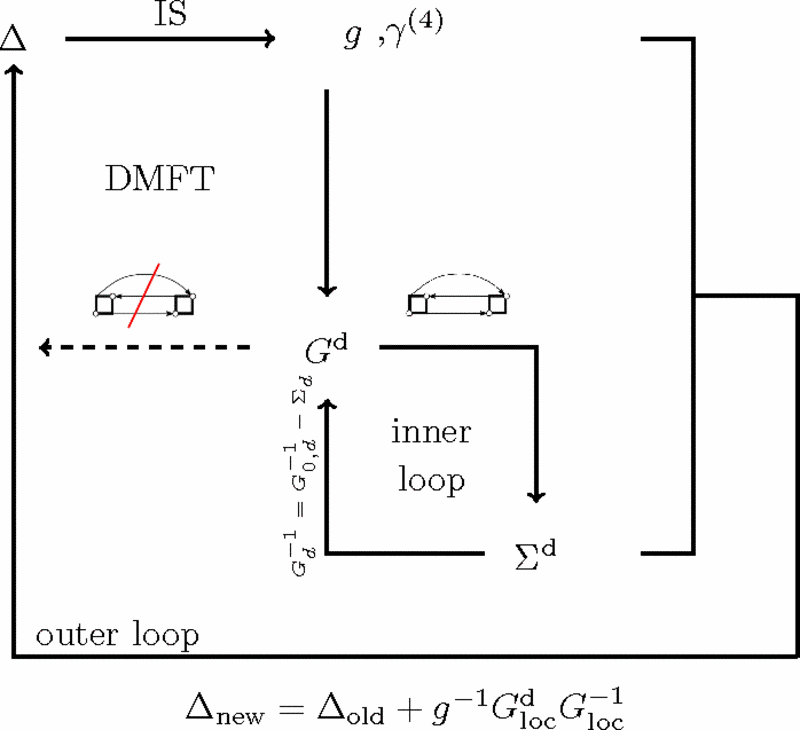
\includegraphics[scale=0.3]{DFcycle}
\caption{Процедура вычислений методом дуальных фермионов}
\label{fig:DFcycle}
\end{figure}

\section{Метод одночастичный неприводимого функционала (1-particle irreducible approach, 1PI)}
В работе \cite{katanin} была рассмотрена другая диаграммная техника, в основном схожая с методом дуальных фермионов, но использующая преобразование Лежандра для введения функционалов $\phi^+$ и $\phi$ от
фермионных полей $\eta^+$,$\eta$ в соответствующую DMFT часть действия (\ref{dual_S}). Также было показано, что диаграммы (например рис. \ref{diag1PI}) в методе 1PI будет содержать поправки к собственной энергии, 
не доступные дуальному методу при использовании лишь двух-частичных вершин, т.е. для их учета необходимы уже трех-частичные вершины.

\begin{figure}[H]
 \centering
 \label{diag1PI}
 \tiny\diagOnePI
\end{figure}

\section{Диаграммы высшего порядка}
\label{section:diags}

Будут рассчитываться две диаграммы. Следуя методу дуальных фермионов строится простейшая диаграмма, содержащая трёх-частичную вершину

\vspace{1cm}

\begin{equation}
\label{diag6}
\begin{tikzpicture}[baseline=-5pt]\node{\diagsixempty};\end{tikzpicture}=
\sum_{\sigma}\left[
\begin{tikzpicture}[baseline=-5pt]\node{\tiny\diagsix{\uparrow}{\uparrow}{\uparrow}{\uparrow}{\uparrow}{\uparrow}{\sigma}{\sigma}{\uparrow}};\end{tikzpicture}+
\begin{tikzpicture}[baseline=-5pt]\node{\tiny\diagsix{\downarrow}{\downarrow}{\uparrow}{\downarrow}{\downarrow}{\uparrow}{\sigma}{\sigma}{\uparrow}};\end{tikzpicture}+
\begin{tikzpicture}[baseline=-5pt]\node{\tiny\diagsix{\uparrow}{\downarrow}{\downarrow}{\uparrow}{\downarrow}{\downarrow}{\sigma}{\sigma}{\uparrow}};\end{tikzpicture}
\right]
\end{equation}

\vspace{1cm}

Следуя методу одно-частичных неприводимых функционалов, диаграмма содержит только двух-частичные вершины

\vspace{1cm}

\begin{equation}
\label{diag3G}
\begin{tikzpicture}[baseline=-5pt]\node{\diagthreeGempty};\end{tikzpicture}=
\begin{tikzpicture}[baseline=-5pt]\node{\tiny\diagthreeG{\uparrow}{\downarrow}{\downarrow}{\uparrow}{\uparrow}{\downarrow}{\uparrow}{diag3G3}};\end{tikzpicture}+
\sum_{\sigma}\left[
\begin{tikzpicture}[baseline=-5pt]\node{\tiny\diagthreeG{\uparrow}{\uparrow}{\uparrow}{\uparrow}{\sigma}{\sigma}{\sigma}{diag3G1}};\end{tikzpicture}+
\begin{tikzpicture}[baseline=-5pt]\node{\tiny\diagthreeG{\uparrow}{\uparrow}{\downarrow}{\downarrow}{\sigma}{\sigma}{\sigma}{diag3G2}};\end{tikzpicture}
\right]
\end{equation}

\vspace{1cm}

По правилам на стр.\pageref{rules} строятся соответствующие формулы для собственной энергии

\begin{equation}
 \tilde{\Sigma}^\text{c}_\omega = (-1)^2 \frac{1}{2!} \frac{1}{N^2} \sum_{\mathbf{k,K}} \beta^{-3}  \sum_{\substack{\omega'\omega''\\\Omega}} \chi_{\substack{\omega\Omega\\\mathbf{K}}}^{(0)}
 \left[
 \Gamma^{\uparrow\uparrow\downarrow\downarrow}_{\substack{\omega\omega'\\\Omega}}  \Gamma^{\uparrow\downarrow\downarrow\uparrow}_{\substack{\omega'\omega''\\\Omega}}  \Gamma^{\downarrow\downarrow\uparrow\uparrow}_{\substack{\omega\omega''\\\Omega}}
 + \sum_{\sigma} \left(
 \Gamma^{\uparrow\sigma\sigma\uparrow}_{\substack{\omega\omega'\\\Omega}}  \Gamma^{\uparrow\uparrow\downarrow\downarrow}_{\substack{\omega'\omega''\\\Omega}}  \Gamma^{\downarrow\sigma\sigma\downarrow}_{\substack{\omega\omega''\\\Omega}}+
 \Gamma^{\uparrow\sigma\sigma\uparrow}_{\substack{\omega\omega'\\\Omega}}  \Gamma^{\uparrow\uparrow\uparrow\uparrow}_{\substack{\omega'\omega''\\\Omega}}  \Gamma^{\uparrow\sigma\sigma\uparrow}_{\substack{\omega\omega''\\\Omega}}
 \right)
 \right]_\mathbf{K}
 \chi_{\substack{\omega''\Omega\\\mathbf{K}}}^{(0)}  G_{\substack{\omega+\Omega\\\mathbf{k+K}}}
\end{equation}

\begin{equation}
 \tilde{\Sigma}^\text{d}_\omega = (-1)^2 \frac{1}{2!} \frac{1}{N} \sum_{\mathbf{K}} \sum_{\sigma}\sum_{\substack{\omega'\omega''\\\Omega}}
 \chi_{\substack{\omega'\Omega'\\\mathbf{K}}}^{(0)} \left[
  \gamma^{(6)\sigma\sigma\uparrow\uparrow\downarrow\downarrow}_{\substack{\omega\omega'\omega''\\\Omega 0}} \gamma^{(4)\uparrow\uparrow\downarrow\downarrow}_{\substack{\omega'\omega''\\\Omega}} +
  \gamma^{(6)\sigma\sigma\uparrow\uparrow\uparrow\uparrow}_{\substack{\omega\omega'\omega''\\\Omega 0}}\gamma^{(4)\uparrow\uparrow\uparrow\uparrow}_{\substack{\omega'\omega''\\\Omega}} +
  \gamma^{(6)\sigma\sigma\downarrow\uparrow\uparrow\downarrow}_{\substack{\omega\omega'\omega''\\\Omega 0}} \gamma^{(4)\uparrow\downarrow\downarrow\uparrow}_{\substack{\omega'\omega''\\\Omega}} 
  \right]_\mathbf{K}
  \chi_{\substack{\omega''\Omega\\\mathbf{K}}}^{(0)}
\end{equation}

\chapter{Ход работы}

\section{Модель}

Гамильтониан $d=2$ примесной задачи без гибридизации
\begin{equation}
\label{hamil}
 H^{\text{imp}} = -\mu(\mathbf{n}_\uparrow+\mathbf{n}_\downarrow) + U\mathbf{n}_\uparrow\mathbf{n}_\downarrow
\end{equation}

В режиме с полузаполнением $\mu = \frac{U}{2}$.

\section{Блоки и линии диаграммы}

Приводимая двух-частичная и трех-частичная функции Грина примесной задачи
\begin{equation}
\begin{split}
\chi_{1234} &= \left<\mathrm{T}\hat{\mathrm{c}}_1\hat{\mathrm{c}}^\dagger_2\hat{\mathrm{c}}_3\hat{\mathrm{c}}^\dagger_4\right>_\text{imp} \\
\chi_{123456} &= -\left<\mathrm{T}\hat{\mathrm{c}}_1\hat{\mathrm{c}}^\dagger_2\hat{\mathrm{c}}_3\hat{\mathrm{c}}^\dagger_4\hat{\mathrm{c}}_5\hat{\mathrm{c}}^\dagger_6\right>_\text{imp}
\end{split}
\end{equation}

Соответствующие неприводимые функции
\begin{equation}
\begin{split}
\gamma^{(4)} = g_{11'}^{-1}g_{22'}^{-1}\left(\chi_{11'22'}+\chi_{12}\chi_{1'2'}-\chi_{12'}\chi_{1'2}\right)g_{33'}^{-1}g_{44'}^{-1}
\\
\begin{aligned}
\gamma^{(6)} & =  g_{11'}^{-1}g_{22'}^{-1} g_{33'}^{-1}g_{44'}^{-1} g_{55'}^{-1}g_{66'}^{-1} ( \chi_{11'22'3'3'} \\
& -2 \chi_{11'} \chi_{22'} \chi_{33'} 
+2 \chi_{11'} \chi_{23'} \chi_{32'}
-2 \chi_{12'} \chi_{23'} \chi_{31'} \\ 
& +2 \chi_{12'} \chi_{21'} \chi_{33'}
-2 \chi_{13'} \chi_{21'} \chi_{32'}
+2 \chi_{13'} \chi_{22'} \chi_{31'} \\
& +\chi_{11'} \chi_{22'33'}
-\chi_{12'} \chi_{21'33'}
+\chi_{13'} \chi_{21'32'} \\
& -\chi_{21'} \chi_{12'33'}
+\chi_{22'} \chi_{11'33'}
-\chi_{23'} \chi_{11'32'} \\
& +\chi_{31'} \chi_{12'23'}
-\chi_{32'} \chi_{11'23'}
+\chi_{33'} \chi_{11'22'}
)
\end{aligned}
\end{split}
\end{equation}

Удобно вместо последовательных временных аргументов использовать интервалы, соответствующие порядку операторов на рисунке \ref{operators}.
Переход к новым переменным осуществляется следующей заменой

\begin{equation}
\begin{split}
\tau_4 \to 0 \\
\tau_3 \to \tau_1 \\
\tau_2 \to \tau_1 - T \\
\tau_1 \to \tau_1 - T + \tau_2
\end{split}
\end{equation}

Что соответствует следующей замене в частотном представлении

\begin{equation}
\begin{split}
\omega_1 \to \omega \\
\omega_2 \to \omega+\Omega \\
\omega_3 \to \omega'+\Omega \\
\omega_4 \to \omega'
\end{split}
\end{equation}

\begin{figure}[H]
\centering
\begin{tikzpicture}
 \draw [->] (0,0) -- (-4,0)
  node[align=center,below,pos=0]{$\tau_4$\\$\mathbf{c}^\dagger$} node[align=center,below,pos=0.25]{$\tau_3$\\$\mathbf{c}$} 
  node[align=center,below,pos=0.5]{$\tau_2$\\$\mathbf{c}^\dagger$} node[align=center,below,pos=0.75]{$\tau_1$\\$\mathbf{c}$} 
  node[below,pos=1]{$\tau$}
  node[above,pos=0.125]{$\tau_1$} node[above,pos=0.375]{$-T$} node[above,pos=0.625]{$\tau_2$};
 \foreach \x in {-3,...,0}
  \draw (\x,1pt) -- (\x,-1pt);
\end{tikzpicture}
\caption{}
\label{operators}
\end{figure}

Линия, в нулевом приближении, равна
\begin{equation}
\begin{split}
&\tilde{G}^{(0)}_{\omega k} = - g^2_\omega(g_\omega-\epsilon^{-1}_k)^{-1},\;\text{где} \\
g_\omega &= \int_0^\beta \mathrm{d}\tau \left(-\left< \mathbf{c}_\uparrow(\tau)\mathbf{c}^\dag_\uparrow(0) \right>\right) e^{i\omega\tau} = \frac{-i\omega}{\omega^2+\mu^2} \\
\epsilon_k &= - 2 t (\cos k_x+\cos k_y).
\end{split}
\end{equation}

Лестничная диаграмма в целом характеризуется волновым вектором $K$ и частотой $\Omega$.

Для удобства две промежуточные линии на диаграммах можно обозначить новой величиной
\begin{equation}
\tilde{\chi}^{(0)}_{\substack{\Omega K\\\omega}} = -\int_k  \tilde{G}_{\omega k} \tilde{G}_{\substack{\omega+\Omega\\k+K}} 
\end{equation}
где суммирование $\sum_\omega$ проводится по мацубаровским частотам $\omega_n = \frac{(2n+1)\pi}{\beta}, n\in\mathbb{Z}$ и $\int_k \equiv \frac{1}{(2\pi)^2}\iint_{-\pi}^{\pi} \mathrm{d}^2k$.

\begin{figure}[H]
\centering
\subfigure[]{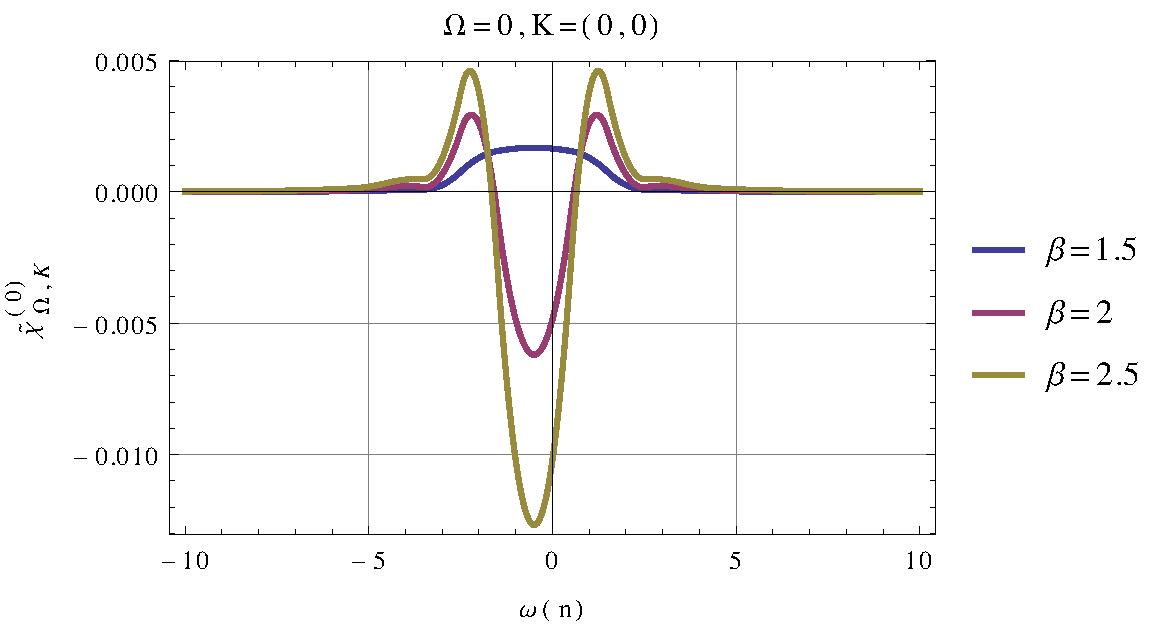
\includegraphics[scale=0.3]{Chi_beta}}
\subfigure[]{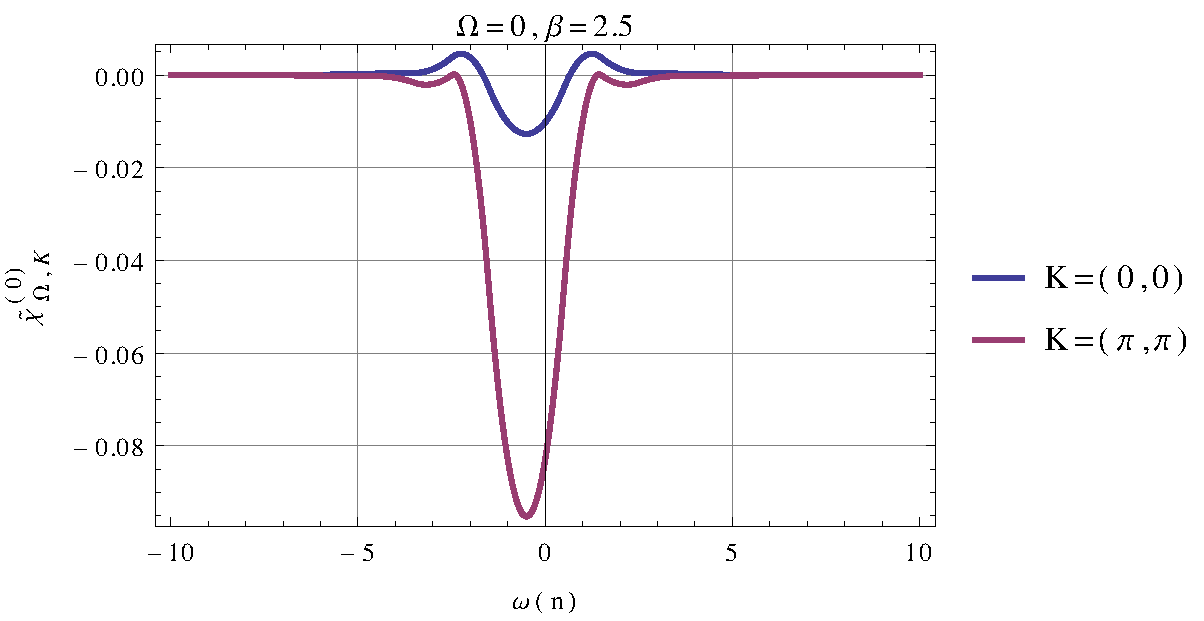
\includegraphics[scale=0.3]{Chi_K}}
\subfigure[]{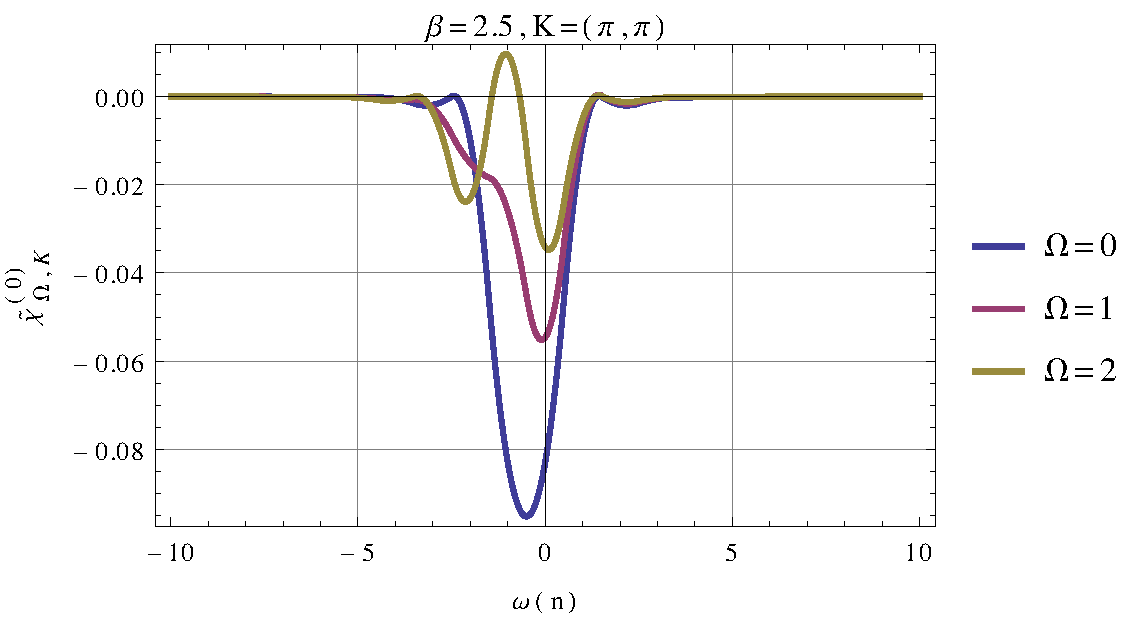
\includegraphics[scale=0.3]{Chi_Omega}}
\caption[]{Зависимости $\tilde{\chi}^{(0)}$ от частоты при различных параметрах}
\end{figure}

Как можно легко заметить $\tilde{\chi}^{(0)}$ быстро затухает с частотой, поэтому в численных расчетах можно ограничиться определенным диапазоном частот $\{-\frac{2N+1}{\beta}\pi,\frac{2N+1}{\beta}\pi\}$, и вне которого $\tilde{\chi}^{(0)} = 0$.

\section{Расчет лестничной диаграммы}

Приведем численный расчет собственной энергии в лестничном приближении.
В атомном пределе, в отсутствии гибридизации $\Delta\equiv 0$ гамильтониан задачи (\ref{hamil}) разрешает аналитическое решение для функций Грина и вершин $\gamma^{(4)}$,$\gamma^{(6)}$. 
Зная выражения для вершин, импульсное и частотное пространство разбиваются на сетки и производится суммирование по соответствующим формула.
Процедура суммирование производится несколько раз, на каждом этапе цикла ``ожирняя'' функцию Грина, что соответствует внутреннему циклу (\ref{fig:DFcycle}) процедуры расчетов в методе дуальных фермионов.

\begin{figure}[H]
\centering
\subfigure[]{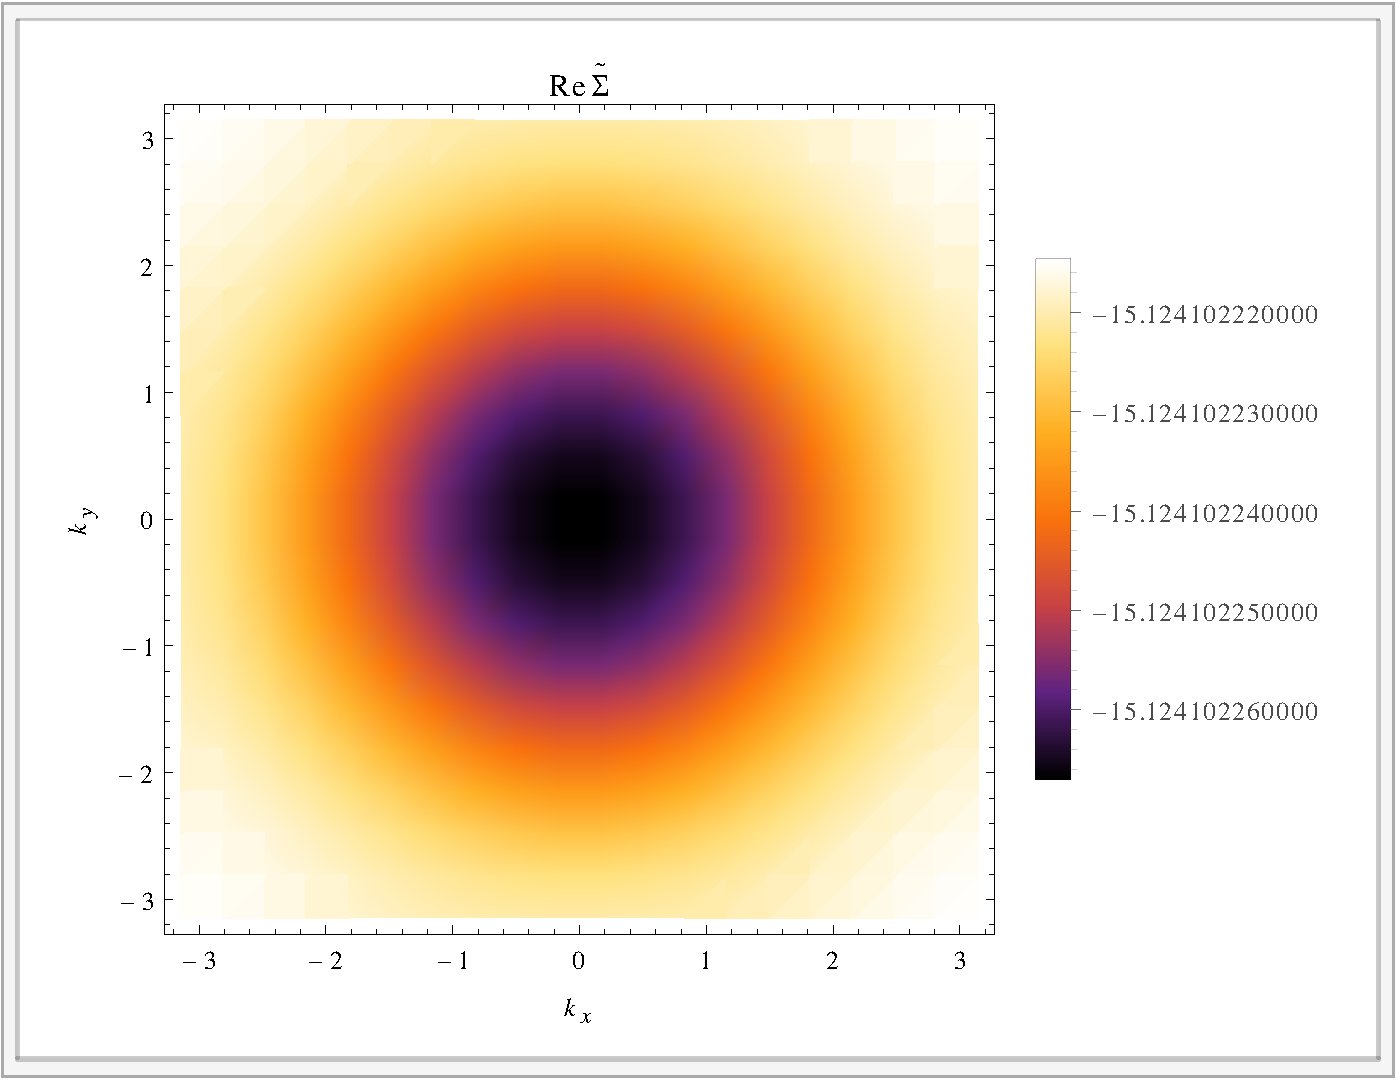
\includegraphics[scale=0.3]{SigmaLDFA_Re}}
\subfigure[]{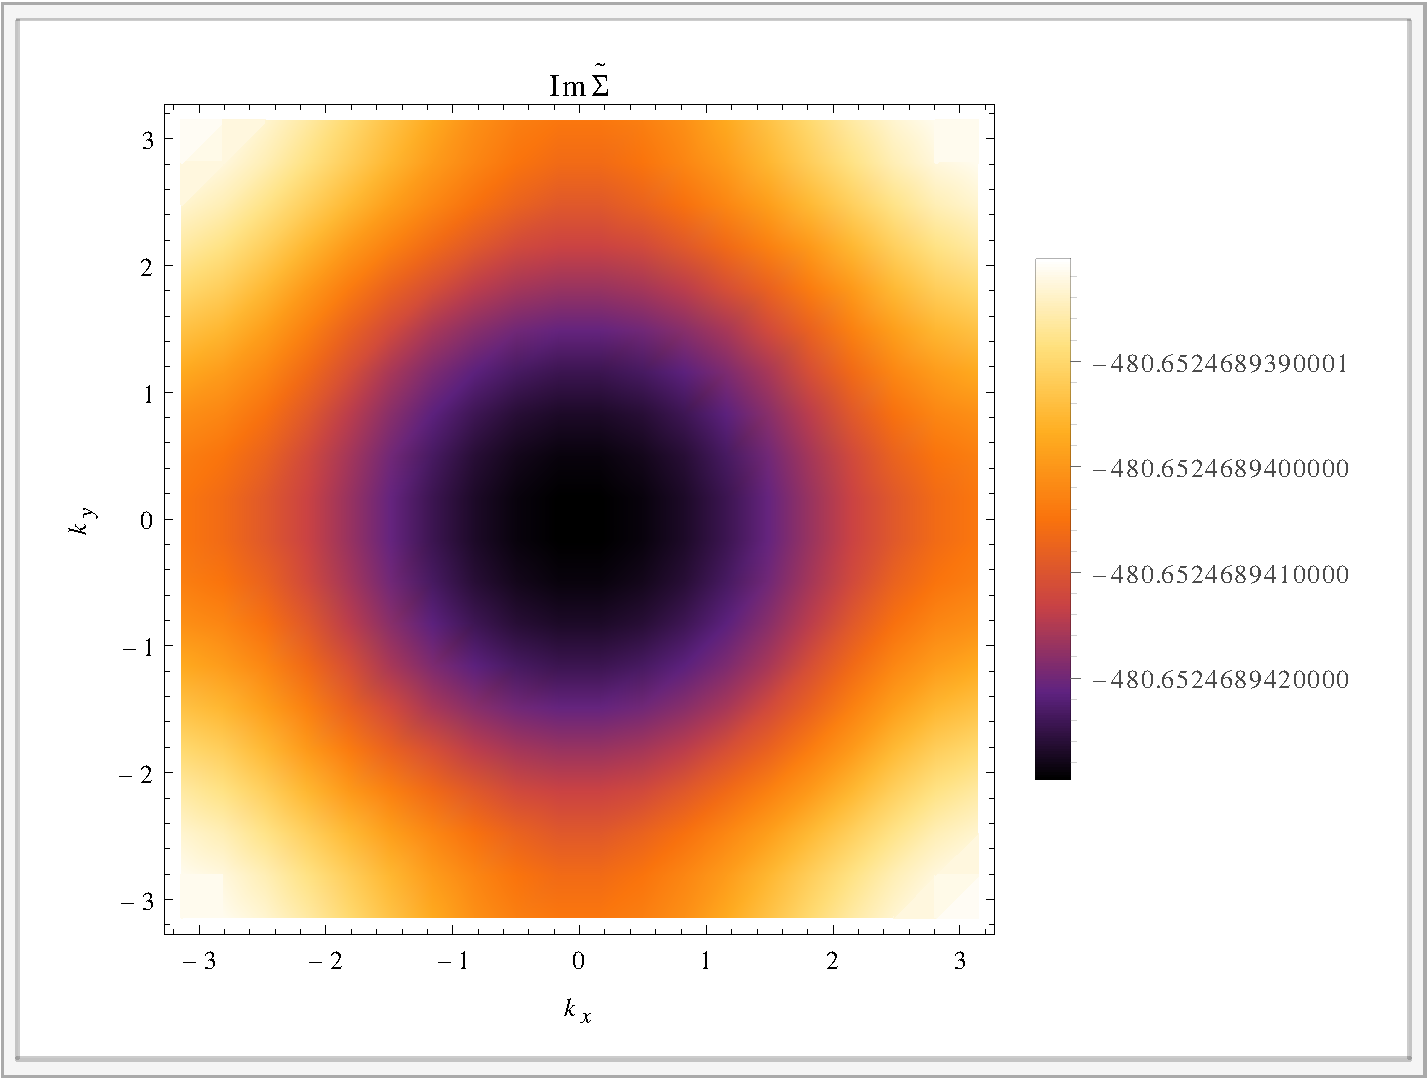
\includegraphics[scale=0.3]{SigmaLDFA_Im}}
\\
\subfigure[]{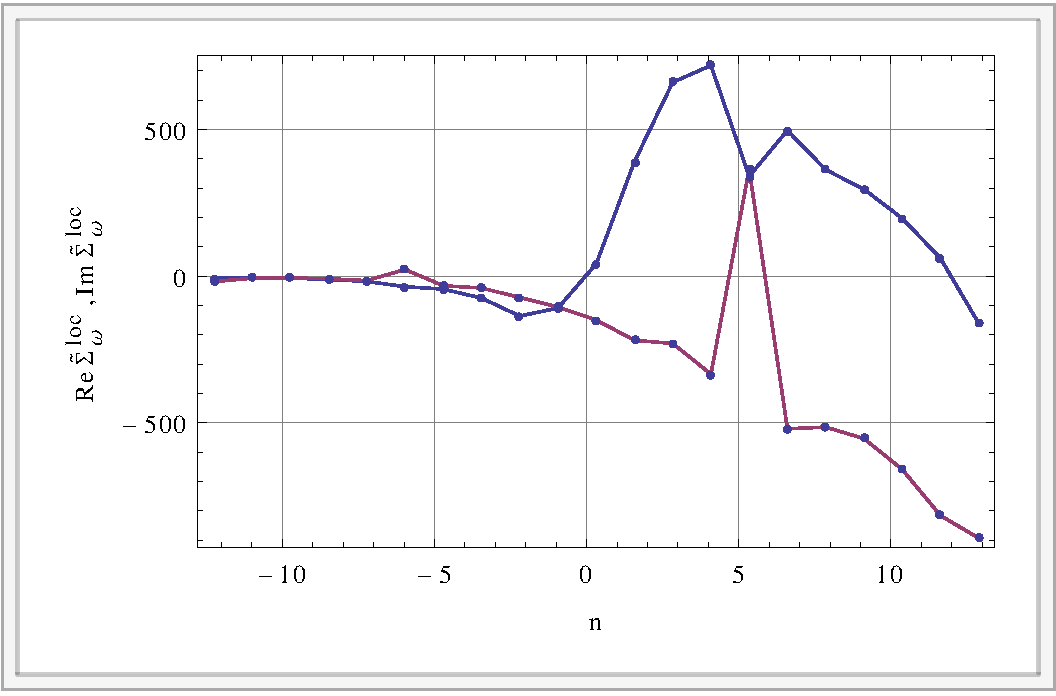
\includegraphics[scale=0.6]{SigmaLDFA}}
\caption{Зависимости действительной и мнимой части собственной энергии в лестничном приближении от импульса (a,b) и от частоты (c) после 30-и итераций цикла. $\beta=10$, $U=4.0$, $t=0.25$}
\label{SigmaLDFA}
\end{figure}

\section{Расчет диаграмм третьего порядка}

Вместе с лестничным приближением, аналогично считаются локальные диаграммы рассмотренные в разделе (\ref{section:diags}).

\begin{figure}[H]
\centering
\subfigure[$Re$]{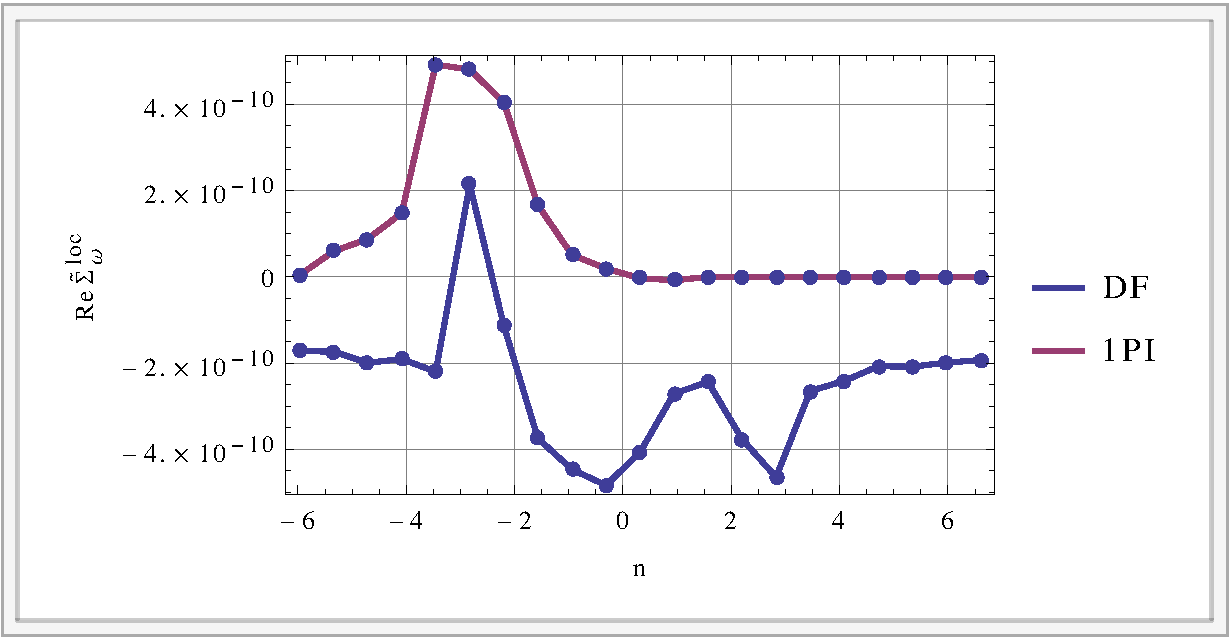
\includegraphics[scale=0.3]{Sigma_Re}}
\subfigure[$Im$]{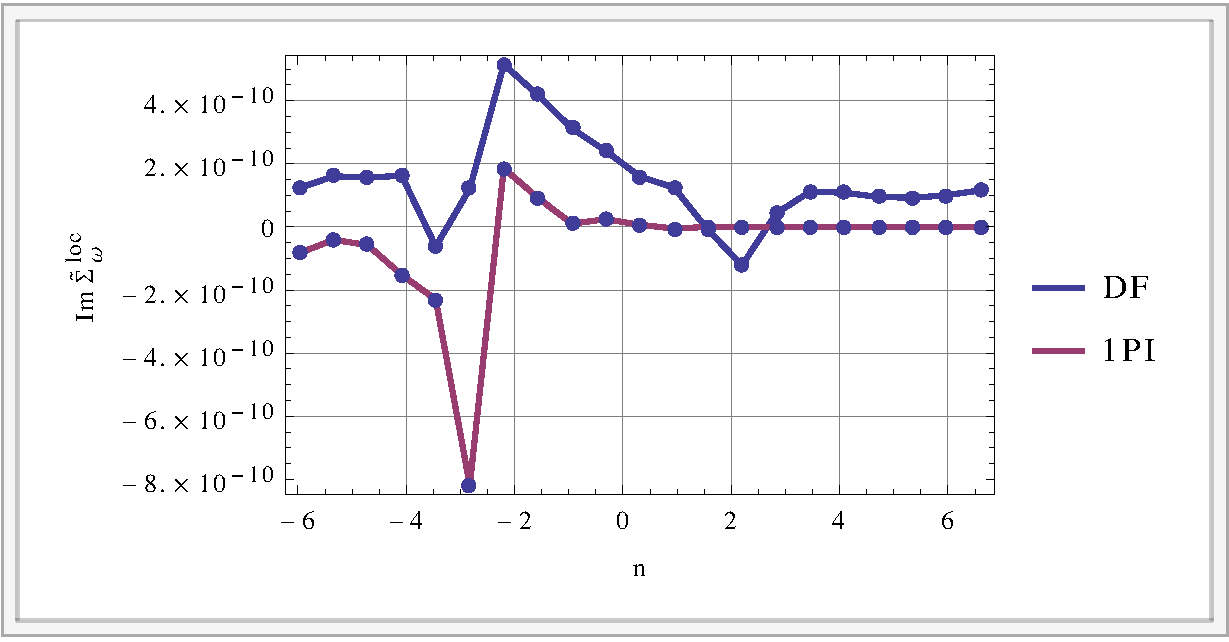
\includegraphics[scale=0.3]{Sigma_Im}}

\caption{Зависимости действительной и мнимой части собственной энергии для двух диаграмм третьего порядка после 30-и итераций цикла. $\beta=10$, $U=4.0$, $t=0.25$}
\label{Sigma}
\end{figure}

\section{Заключение}



%Делаем Фурье преобразования
%
%\begin{equation}
%\begin{split}
%X_{\substack{\Omega K\\ \tau\tau'}} &= 
%  \chi_{\substack{\Omega\\ \tau\tau'}} + \beta^{-3} \sum_{\omega\omega'\omega''}\chi_{\substack{\Omega\\\omega\omega''}}X^{(0)}_{\substack{\Omega K\\\omega''}}X_{\substack{\Omega K\\\omega''\omega'}}e^{-i\omega\tau}e^{-i\omega'\tau'}\\
% &= \chi_{\substack{\Omega\\ \tau\tau'}} + \beta^{-1}\sum_{\omega''}\chi_{\substack{\Omega\\\tau\omega''}}X^{(0)}_{\substack{\Omega K\\\omega''}}X_{\substack{\Omega K\\\omega''\tau'}}\\
% &= \chi_{\substack{\Omega\\ \tau\tau'}} + \beta^{-1}\sum_{\omega''}\chi_{\substack{\Omega\\\tau\omega''}}X^{(0)}_{\substack{\Omega K\\\omega''}}\left(\int_{\tau''}X_{\substack{\Omega K\\\tau''\tau'}}e^{i\omega''\tau''}\right)\\
% &= \chi_{\substack{\Omega\\ \tau\tau'}} + \int_{\tau''}\left(\beta^{-1}\sum_{\omega''}\chi_{\substack{\Omega\\\tau\omega''}}X^{(0)}_{\substack{\Omega K\\\omega''}}e^{i\omega''\tau''}\right)X_{\substack{\Omega K\\\tau''\tau'}}\\
% \beta^{-1}\sum_{\omega''}\chi_{\substack{\Omega\\\tau\omega''}}X^{(0)}_{\substack{\Omega K\\\omega''}}e^{i\omega''\tau''}
%  &= \beta^{-1}\sum_{\omega''}\left(\int_{\tilde{\tau}''}\chi_{\substack{\Omega\\\tau\tilde{\tau}''}}e^{i\omega''\tilde{\tau}''}\right)X^{(0)}_{\substack{\Omega K\\\omega''}}e^{i\omega''\tau''}
%   = \int_{\tilde{\tau}''}\chi_{\substack{\Omega\\\tau\tilde{\tau}''}}X^{(0)}_{\substack{\Omega K\\-\tilde{\tau}''-\tau''}}
%\end{split}
%\end{equation}
%
%Для вычисления $X^{(0)}_{\substack{\Omega K\\-\tilde{\tau}''-\tau''}}$ понадобятся граничные условия периодичности
%\begin{equation}
%  X_{\beta+\tau} = -X_{\tau} = -X_{-\tau}
%\end{equation}
%
%Получаем интегральное уравнение
%
%\begin{equation}
%\begin{split}
%X_{\substack{\Omega K\\ \tau\tau'}} - 
%  \int_0^\beta\mathrm{d}\tau''\underbrace{\left(\int_{\tilde{\tau}''}\chi_{\substack{\Omega\\\tau\tilde{\tau}''}}X^{(0)}_{\substack{\Omega K\\-\tilde{\tau}''-\tau''}}\right)}_{A_{\tau\tau''}}X_{\substack{\Omega K\\\tau''\tau'}}
%  = \chi_{\substack{\Omega\\ \tau\tau'}}
%\end{split}
%\end{equation}
%
%Образуем сетку $N\times N$ по $\tau$-переменным: $\tau_i=i\Delta\tau, i\in \overline{0,N}$, где $\Delta\tau=\frac{\beta}{N}$, тогда интегральное уравнение
%можно будет заменить на систему $(N+1)^2$ линейных уравнений c $(N+1)^2$ неизвестными
%
%\begin{equation}
% X_{ij} - \sum_{k=0}^N a_{ik}X_{kj} = b_{ij}
%\end{equation}
%
%где $X_{ij} = X_{\substack{\Omega K\\ \tau_i\tau_j}}, a_{ik} = \int_\tau\chi_{\substack{\Omega\\\tau_i\tau}}X^{(0)}_{\substack{\Omega K\\-\tau-\tau_k}},b_{ij}=\chi_{\substack{\Omega\\ \tau_i\tau_j}}$

\newpage
\nocite{*}
\bibliographystyle{plain}
\bibliography{bibliography}

\end{document}